\section{Task 1}
\label{sec:task1}
\textit{Make a Uppaal model of it and generate a feasible schedule.}\\\\
The problem can be modelled in several different ways, some more general than others. By \textit{general} we mean their ability to be easily modified to fit other similar problems. In our solution the model is relatively specific to the problem we are solving, as making it more general would take us too much time. In other words, if we want to change something in our model, we have to change it in several places.

We will explain our model from the templates, and include an explanation of the declarations from that. The model consists of 7 templates, but only 3 of them are significantly differnet, so we will use these 3 to explain the entire model. The first template is the boat, as shown in \Cref{fig:boat}.

\begin{figure}[H] \centering
	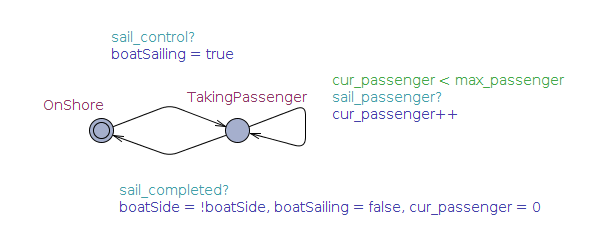
\includegraphics[width=1\textwidth]{Images/boat.png}
	\caption{The \textit{Boat} template.}\label{fig:boat}
\end{figure} 

\noindent The initial location, \texttt{OnShore}, has an edge that synchronizes with the people who can sail the boat, on the channel \texttt{sail_control} and moves to the location \texttt{TakingPassenger}. Here we have two options: The first is to ynchronize with a passenger on the channel \texttt{sail_passenger}, this can be any person on the same shore as the boat. This edge has a guard, making sure that our current number of passengers, \texttt{curr_passenger}, is less than the max allowed amount, \texttt{max_passenger} (for this assignment \texttt{max_passenger} is 1). If the synchronization is successful \texttt{cur_passenger} is incremented. The other is to synchronize with the person who controls the boat on the broadcast channel \texttt{sail_completed}, which also synchronizes with the passenger and results in both controller and passenger being moved to the other side. It also changes the side of the boat and resets the \texttt{cur_passenger} variable.

\begin{figure}[H] \centering
	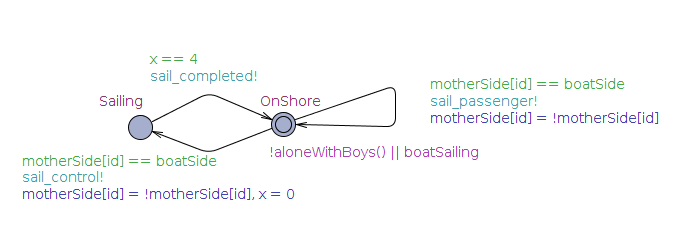
\includegraphics[width=.9\textwidth]{Images/mom.png}
	\caption{The \textit{Mother} template.}\label{fig:mother}
\end{figure} 

\noindent \Cref{fig:mother} shows the template for the Mother, which is very similar to the one for the Father and Police Officer - only the names differ, and the Police Officer does not have an invariant on the initial location. From the initial location, \texttt{OnShore} there are two options.

The first is to synchronize with the boat on \texttt{sail_control}, and this edge has a guard making sure the mother is on the same side as the boat; if successful we move to the \texttt{OnBoat} location, and the boat moves to a state where it accepts passengers. In this location we wait to synchronize with the boat on \texttt{sail_completed}, change the side of the mother, and move back to the \texttt{OnShore} location - that is, if the invariant \texttt{!aloneWithBoys()} is not violated; if that happens it will result in a deadlock. This could be solved by adding an option to unload people from the boat instead of synchronizing with \texttt{sail_completed}, but this is not necessary to find the most efficient solution, as simulations that end in a deadlock can be discarded; it clearly does not make sense to load and unload the boat on the same shore, when we are looking to be efficient. 

The second option is for the mother to be a passenger, and synchronize with the boat on \texttt{sail_passenger}. Again we check that the mother is on the same side as the boat, and assuming everything is okay we synchronize again on \texttt{sail_completed}, and change sides.

The \texttt{x} variable is a clock which is needed for \texttt{Task 2} (\Cref{sec:task2}).

\begin{figure}[H] \centering
	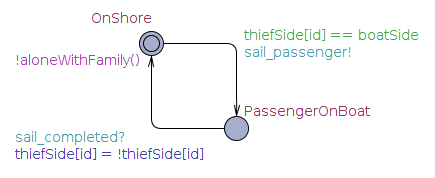
\includegraphics[width=.7\textwidth]{Images/thief.png}
	\caption{The \textit{Thief} template.}\label{fig:thief}
\end{figure} 

\noindent \Cref{fig:thief} shows the template for the thief and the children, only the children do not have the \texttt{!aloneWithFamily()} invariant. The only thing possible here is to synchronize on \texttt{sail_passenger}, check that the thief is on the same side as the boat, synchronize with \texttt{sail_completed}, and change sides.

\subsection{Schedule}
To find a schedule we run the following query through the verifier:\\

\noindent {\footnotesize \texttt{E<> forall(i:mother_t) motherSide[i] == true and forall(i:girl_t) girlSide[i] == true\\
 and forall(i:father_t) fatherSide[i] == true and forall(i:boy_t) boySide[i] == true \\
 and forall(i:police_t) policeSide[i] == true and forall(i:thief_t) thiefSide[i] == true}}\\

\noindent where \texttt{mother_t} is defined as:\\

\texttt{typedef int[0, numMothers-1] mother_t;}\\

\noindent and the other types are defined in a similar fashion.

We asked Uppaal to give us the shortest path, and we got the following result ($\rightarrow$ means the boat goes to the other shore, $\leftarrow$ means it goes back to the starting shore):

\begin{table}[h]
\begin{tabular}{lll}
Police, & Thief & $\rightarrow$ \\
Police & & $\leftarrow$ \\
Police, & Girl 1 & $\rightarrow$ \\
Police, & Thief & $\leftarrow$ \\
Mother, & Girl 2 & $\rightarrow$ \\
Mother &  & $\leftarrow$ \\
Mother, & Father & $\rightarrow$ \\
Father & & $\leftarrow$ \\
Police, & Thief & $\rightarrow$ \\
Mother & & $\leftarrow$ \\
Father, & Mother & $\rightarrow$ \\
Father & & $\leftarrow$ \\
Father, & Boy 1& $\rightarrow$ \\
Police, &  Thief & $\leftarrow$ \\
Police, & Boy 2 & $\rightarrow$ \\
Police & & $\leftarrow$ \\
Police, & Thief & $\rightarrow$ \\
\end{tabular}
\end{table}

\noindent It is clear to see that it does not matter which of the two girls (or boys) go over first, and also that it is possible to switch boys/girls and father/mother giving essentially the same schedule.
